%   MSc Business Analytics Dissertation
%
%   Title:     Aaa Bbbbbbb Cccccccccc
%   Author(s): Xxxxxx Xxxxxxxxx and Yyy Yyyyyyyyy
%
%   Chapter 6: Discussion
%
%   Change Control:
%   When     Who   Ver  What
%   -------  ----  ---  --------------------------------------------------------------
%   11Feb11  AB    0.1  Begun 
%

\chapter{Discussion}\label{C.Discussion}
\section{Introduction}\label{S.Discussion.intro}
\begin{center}
\begin{figure}[!htb]
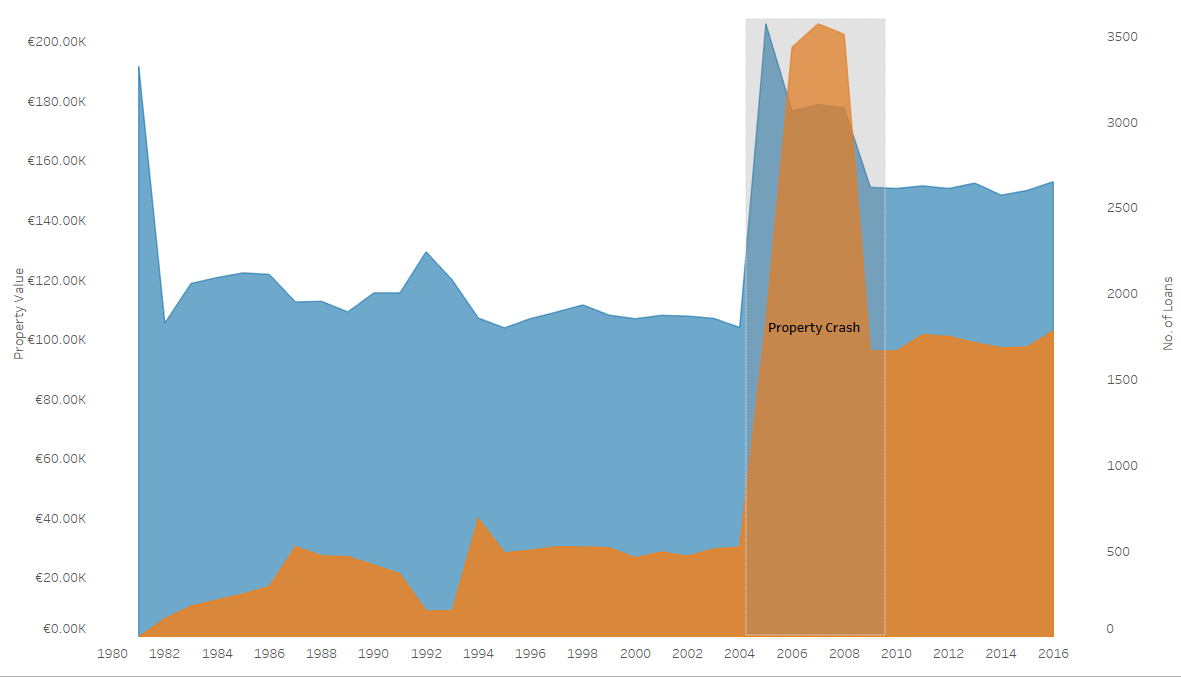
\includegraphics[scale=0.3]{crash1.png}
\centering
\caption{Irish Property Crash}{\textbf{Source:} Tableau Professional v10}
\label{fig:crash1}
\end{figure}
\end{center}
This chapter presents the detailed discussion and analysis of patterns and trends discovered during this research work. Keeping the interest of every stakeholder from bank officer to auditors, an attempt has been build simplicity in the business dashboard so that end user can use it efficiently to drive the business decision. When it was discovered that original data is not appropriate from the predictive modelling perspective, the modified data has been used throughout this research work. All analysis has been presented considering modified data set.

\section{Patterns \&  Analysis}

Since the property crash (2007-2010) average property price and the number of loan applications has been reduced as it can be seen in fig \ref{fig:crash1}. Earlier the average property was \euro 120K then it increased by 100\%.

\begin{center}
\begin{figure}[!htb]
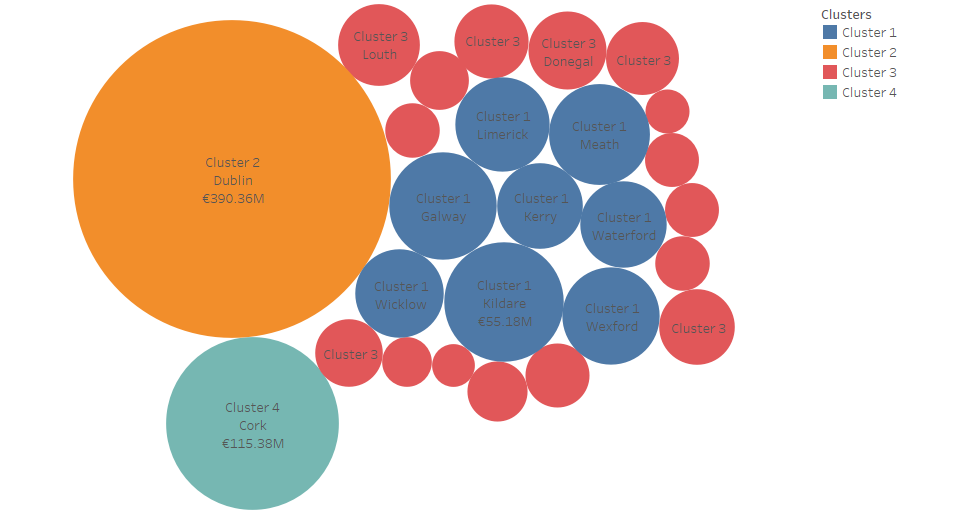
\includegraphics[scale=0.4]{clustero.png}
\centering
\caption{County Cluster}{\textbf{Source:} Tableau Professional v10}
\label{fig:clustero}
\end{figure}
\end{center}

The k-mean algorithm is used to cluster twenty-six(26) counties among four clusters based on the loan balance, as Ireland property market vary a lot in a county. Co. Dublin is classified into cluster \#2, and Co. Cork is classified into cluster \#4 has highest outstanding loan balance. As shown in fig. \ref{fig:cluster} 8 counties are in cluster \#1 and 16 counties with least outstanding loan balance classified into cluster \#3.

\begin{center}
\begin{figure}[!htb]
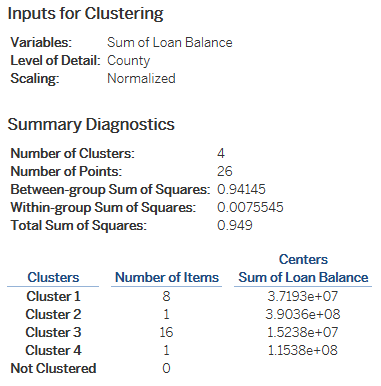
\includegraphics[scale=0.5]{cluster.png}
\centering
\caption{Clustering Results}{\textbf{Source:} Tableau Professional v10}
\label{fig:cluster}
\end{figure}
\end{center}

During data analysis phase, it was noted that the most properties have LTV(Loan-to-value) ratio between 60 - 80\%. There are few properties with LTV higher than 100\%.
In fig. \ref{fig:ltv}
\begin{center}
\begin{figure}[!htb]
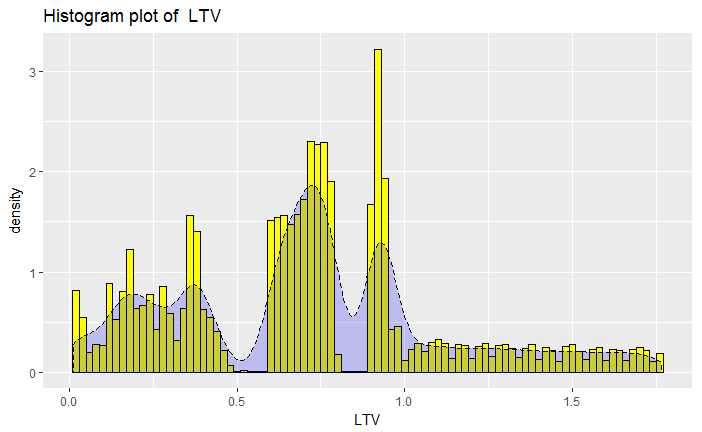
\includegraphics[scale=0.5]{ltv.png}
\centering
\caption{Loan to Value histogram}{\textbf{Source:} R Studio ggplot()}
\label{fig:ltv}
\end{figure}
\end{center}

\begin{center}
\begin{figure}[!htb]
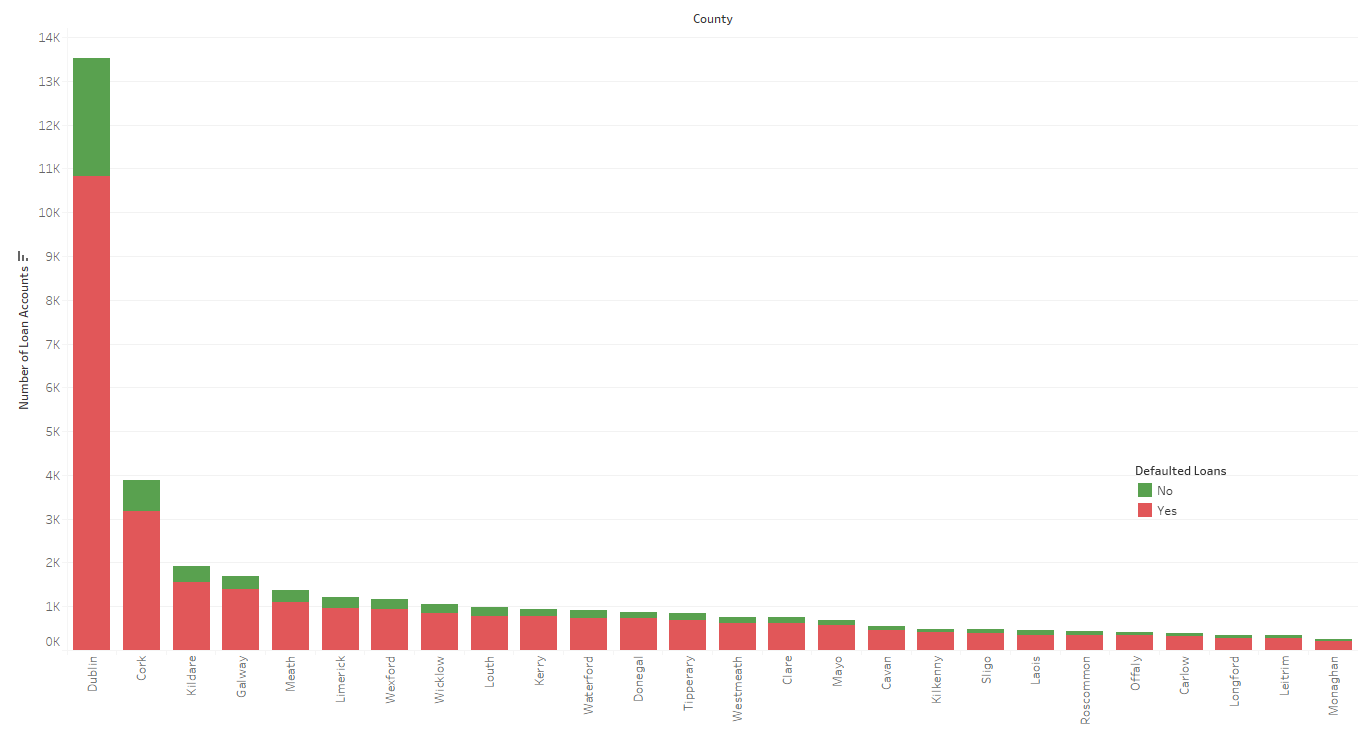
\includegraphics[scale=.4]{countynumber.png}
\centering
\caption{Number of account county wise}{\textbf{Source:} Tableau Pro}
\label{fig:tableaucounty}
\end{figure}
\end{center}

A total number of accounts in the normalised data set was 273,000, and most numbers of default and loan account were from County Dublin and Cork as seen in fig. \ref{fig:tableaucounty}.

\section{Statistical Analysis}

Descriptive analysis has been performed using SPSS tool to get a better understanding of data and take required steps for data preprocessing. It can be seen from fig.\ref{fig:stats1} and fig.\ref{fig:stats2}, there are no missing values or unknown values present in the data as it is very well structured. Statistical analysis helped in generating the rules to normalise data for building an unbiased predictive model. $Loan Balance$ is of 6 digits (e.g. \euro103,584), and $Annual Payment$ is of 4 digits (e.g. \euro4614); in such scenarios, a predictive model can assign more weight to $Loan Balance$ as it is more significant compared to the $Annual Payment$. So, the model will outweigh $Loan Balance$ over $Annual Payment$ but for credit assessment both the variables hold equal importance. Therefore, its is necessary to scale the variables in data set accordingly to achieve better performance.  

\begin{center}
\begin{figure}[!htb]
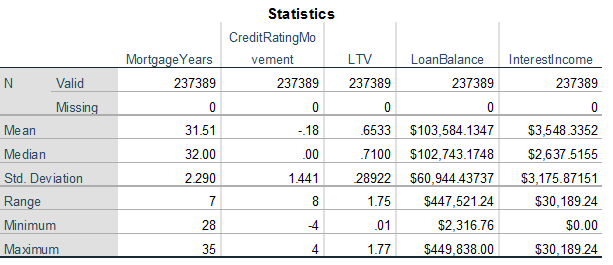
\includegraphics[scale=0.7]{stats1.png}
\centering
\caption{Analysis of Significant variables - 1}{\textbf{Source:} SPSS}
\label{fig:stats1}
\end{figure}
\end{center}


\begin{center}
\begin{figure}[!htb]
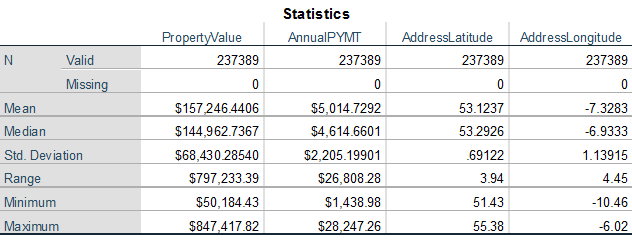
\includegraphics[scale=0.7]{stats2.png}
\centering
\caption{Analysis of Significant variables - 2}{\textbf{Source:} SPSS}
\label{fig:stats2}
\end{figure}
\end{center}



\section{Dashboard}
Considering the day-to-day requirement of stakeholders at KPMG, three business dashboards are designed using Tableau software. Main response to build the dashboard using Tableau, as it allows the easy integrations with the predictive model from R engine and provides a better means to visualise prediction and forecast.

\begin{center}
\begin{figure}[!htb]
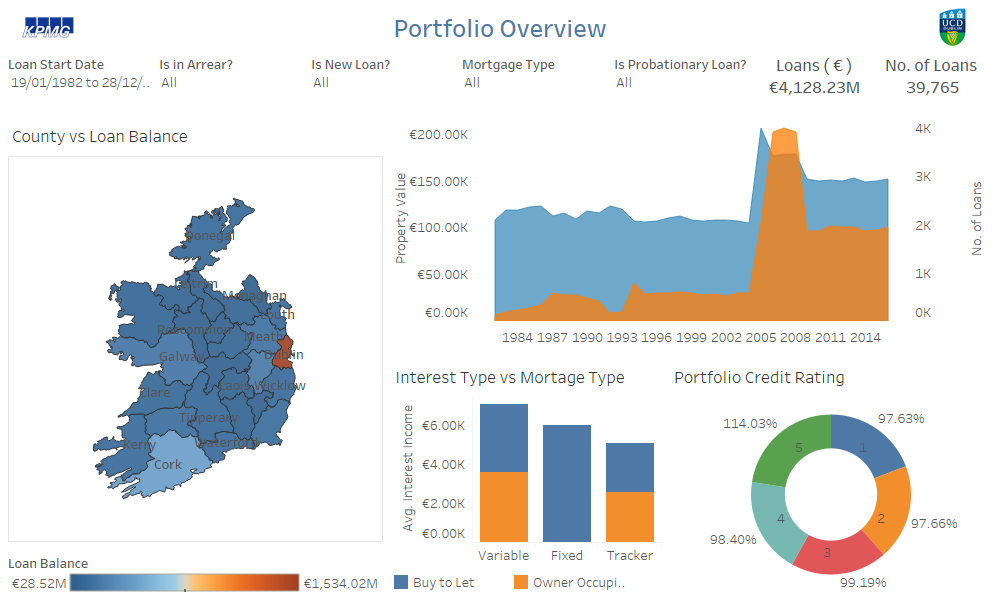
\includegraphics[width=\textwidth]{Overview.png}
\centering
\caption{Portfolio Overview}{\textbf{Source:} Tableau Professional v10}
\label{fig:overview}
\end{figure}
\end{center}


\textbf{Portfolio Overview}\\
Portfolio overview dashboard is built to allow auditors and credit analysts to analyse overall existing loan portfolio registered under a bank. This dashboard allows the user to perform a detailed analysis by selecting various combinations of variables from filters such as:
\begin{itemize}
\item Loan Start Date: User can view a selective number of loan account based on the start date of an account
\item Is in Arrears?: Does a loan account has any outstanding repayment in last one year?
\item Mortgage Type: For what purpose mortgage has been buy-to-let or owner occupied?
\item Is probationary Loan?: Has the loan account been converted to probationary loan
\end{itemize}

The geospatial map allows the analyst to view loan balance for each county, along with a time-series analysis of property price and a number of accounts for past three decades. Using interest type vs mortgage type user can identify which type of interest is giving more income to banks.

\begin{center}
\begin{figure}[!htb]
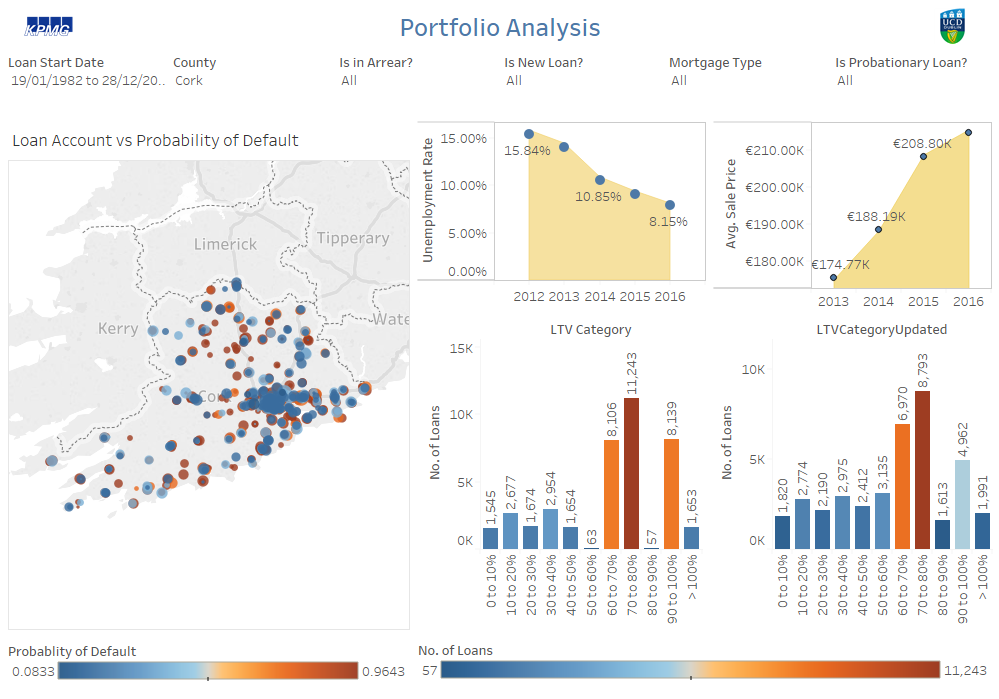
\includegraphics[width=\textwidth]{Analysis.png}
\centering
\caption{Portfolio Analysis}{\textbf{Source:} Tableau Professional v10}
\label{fig:overview}
\end{figure}
\end{center}
\textbf{Portfolio Analysis}\\
Portfolio analysis dashboard allow user to view loan account movement from one LTV (loan to value) category to other, along with unemployment rate and average property sale price in a town. User can select range of property from map using a distance(radius in kms as in fig \ref{fig:dist}) to compare trends in selected neighbourhood.

\begin{center}
\begin{figure}[!htb]
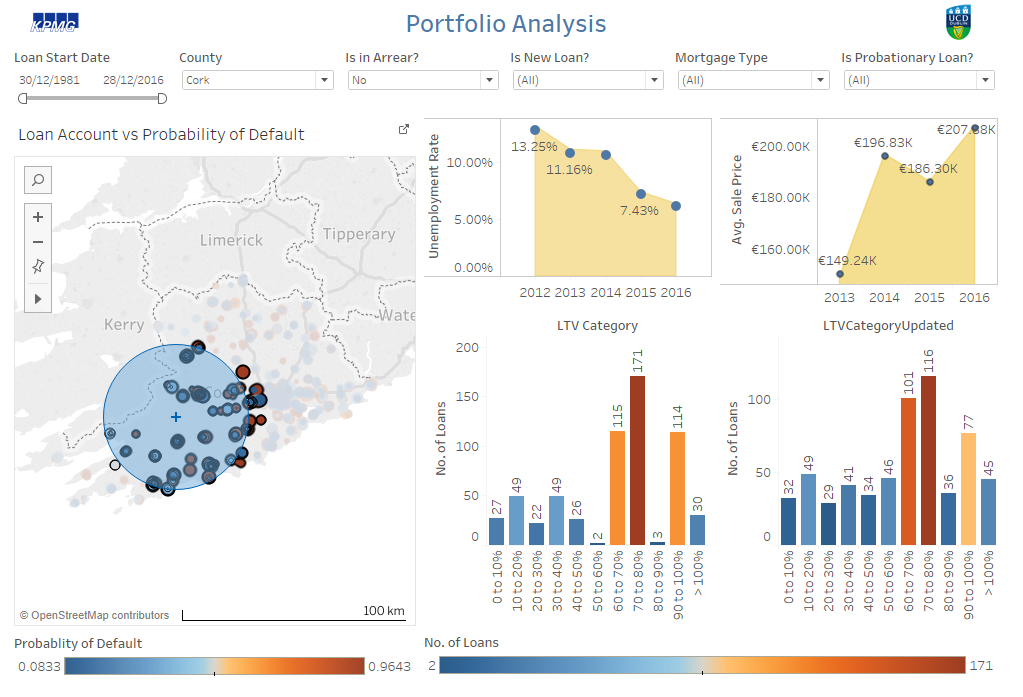
\includegraphics[width=\textwidth]{dist.png}
\centering
\caption{Property Selection using distance}{\textbf{Source:} Tableau Professional v10}
\label{fig:dist}
\end{figure}
\end{center}

\textbf{R Shiny Dashboard}
The second dashboard has been built using R shiny package, which allows one to create interactive dashboards. R shiny is quite a popular package among data scientist as it is open source and easy to deploy. However, only limitations it has that user won't be able to load large datasets, and during this research work, it was observed that dashboard performance was slow data set has more than 100,000 row. A dynamic dashboard has been build which allows user to view property based on clustering and it allows user can view street level statistical metrics as seen in fig \ref{fig:rmap}.

\begin{center}
\begin{figure}[!htb]
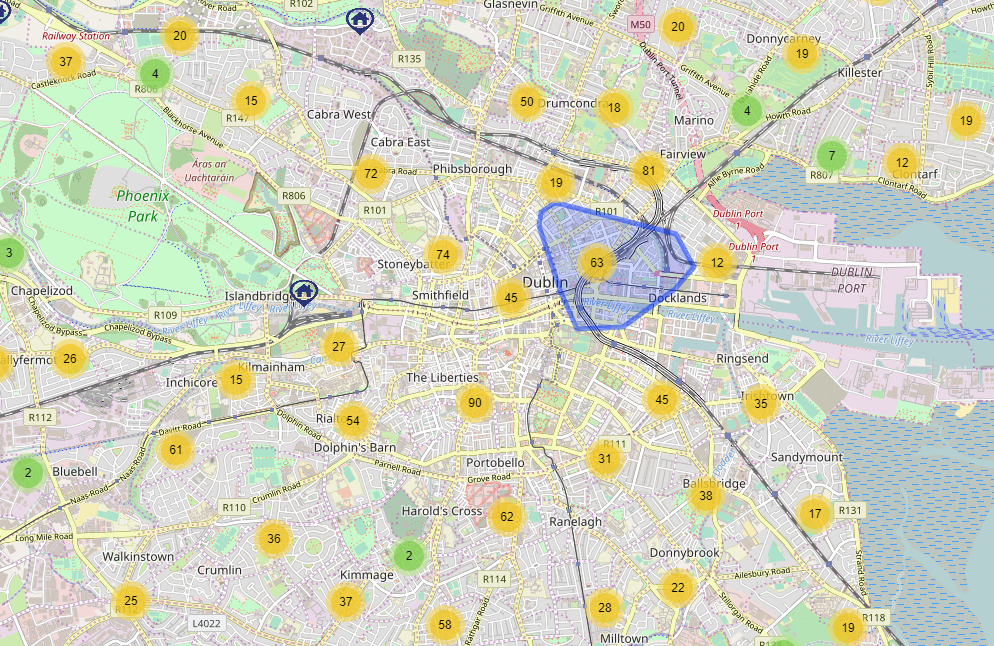
\includegraphics[width=\textwidth]{rmap.png}
\centering
\caption{Dashboard Build using R Shinny}{\textbf{Source:} R Studio}
\label{fig:rmap}
\end{figure}
\end{center}



\section{Success}\label{S.succes}
To measure the performance of this work, a working business dashboard has been given to stakeholders to perform analysis and provide their feedback. The questionnaire covers all qualitative and quantitative measures which focus on the performance of the model, characteristics of a good visualisation, financial aspects and legal information. Based on the feedback received and suggestions dashboard features are improved to satisfy the user needs. The user was given three dashboard designs and asked to recommend best one with possible changes stating the reason for choice made and suggestions to further improve usability.\\

Following represents the overall feedback received from users: 
\begin{itemize}
\item \textbf{47\%}Auditors feel this dashboard is handy
\item \textbf{70\%}Feel that Geospatial techniques have enhanced credit assessment
\item \textbf{60\%}Likely to recommend this dashboard to colleagues
\item \textbf{65\%}Feel that dashboard is very appealing
\end{itemize}

Auditors, Credit Analysts, Data Scientists and Tableau Consultants have responded to the survey by providing unbiased and specific suggestions on all three dashboards. From the recorded responses, it is significant that dashboards are helpful for credit analysis or for making new bank sales strategies. Fig.\ref{fig:feed} represents overall positive or negative responses to the feedback. \\

% Please add the following required packages to your document preamble:
% \usepackage{booktabs}
\begin{table}[!htb]
\centering
\caption{Overall Recorded Response}
\label{fig:feed}
\begin{tabular}{@{}lll@{}}
\toprule
\# & Answer                        & \%      \\ \midrule
1  & Extremely positive            & 37.50\% \\
2  & Moderately positive           & 50.00\% \\
3  & Slightly positive             & 12.50\% \\
4  & Neither positive nor negative & 0.00\%  \\
5  & Slightly negative             & 0.00\%  \\
6  & Moderately negative           & 0.00\%  \\
7  & Extremely negative            & 0.00\%  \\
   & Total                         & 100\%   \\ \bottomrule
\end{tabular}
\end{table}